% $Id: reuse.tex 12369 2010-09-28 08:34:59Z markus $
% Local Variables:
% ispell-check-comments: nil
% Local IspellDict: american
% End:
% --------------------------------------------------------
% User documentation
% copyright by BREDEX GmbH 2004
% --------------------------------------------------------
\app{} lets you reuse (reference) \gdprojects{} as libraries of \gdcases{} in other \gdprojects{}. 

This is different to importing \gdcases{} from an existing \gdproject{} \bxpref{ImportTestCases}, because reused \gdprojects{} are not a copy of the original \gdproject{}, but a reference. Any changes made in the original \gdproject{} will be carried through to places where this \gdproject{} has been reused. 

To reuse \gdprojects{} in \app{}:
\begin{enumerate}
\item Make sure that the \gdproject{} you want to reuse is in the \gddb{}.
\item Select:\\
\bxmenu{Test}{Properties}{}\\
and select \bxname{Used Projects} from the tree on the left of the dialog that appears (\bxfigref{reuseproject}).

\begin{figure}[h]
\begin{center}
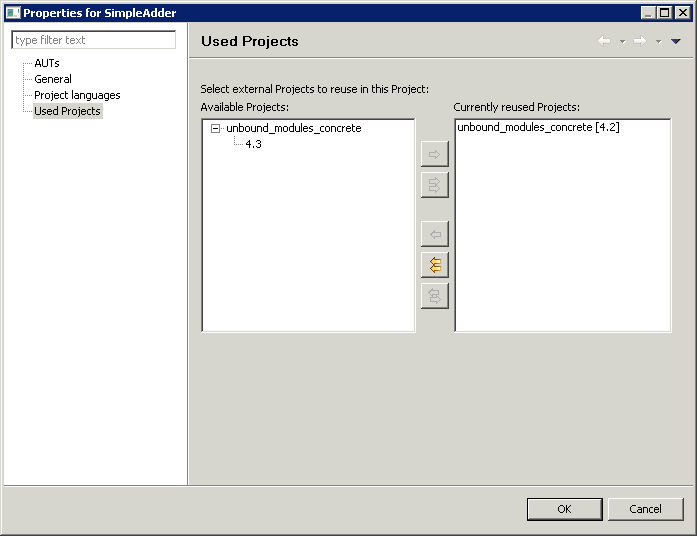
\includegraphics[width=12.5cm]{Tasks/Projects/PS/reuseproject}
\caption{Reused \gdprojects{}}
\label{reuseproject}
\end{center}
\end{figure}

\item A list of \gdprojects{} you can reuse will be offered on the left-hand side of the dialog. You can only reuse \gdprojects{} which support the same toolkit as your current \gdproject{} (e.g. Swing, Concrete).
\bxtipp{To be able to reuse a \gdproject{}, you must have checked the \bxname{reusable} box in the \gdproject{} properties for the \gdproject{} \bxpref{ProjPropertiesGeneral}.}

\item From the list of reusable \gdprojects{}, select a \gdproject{} and its version to reuse in the current \gdproject{}. Use the arrows to move it to the list of reused \gdprojects{}.
\item Click \bxcaption{OK}. 
\item The \gdcases{} from the \gdproject{} you chose to reuse will appear in the \gdtestcasebrowser{}, under a category with the same name as the reused \gdproject{}. The \gdcases{} will be colored blue to distinguish them from other \gdcases{} in this \gdproject{}. 

\bxtipp{You cannot edit these \gdcases{} here -- but you can reuse them in your \gdcases{} for this \gdproject{} and edit certain details (referenced parameters, component names) when they are reused in other \gdcases{}.}
\item You can change the version of the reused \gdproject{} via the \bxname{Used Projects} Properties dialog, by clicking on the \bxcaption{change used version} button \bxpref{changingreusedprojectversion}.
\end{enumerate}

\subsubsection{Changing the version of a reused \gdproject{}}
\gdhelpid{databaseMigrationAssistantContextId}{Datebase Migration}
\label{changingreusedprojectversion}
\gdhelpid{projectUsedPropertyPageContextId}{Used Projects Properties} 
You can change the version of the reused \gdproject{} you are using in your tests. This is useful to update to a new version of the unboud modules, for example. 
\begin{enumerate}
\item In the \bxname{Used \gdproject properties}, select the currently reused \gdproject{} version from the list on the right. 
\item Select the new version of this \gdproject{} from the list on the left. 
\bxtipp{In order to be able to see and select the new version of the \gdproject{}, it must be in your \gddb{}!}
\item Click the \bxcaption{Switch version} button, marked with the opposing arrows. 
\item The version of the reused \gdproject{} will be switched. 
\bxtipp{If changes have taken place, it may be necessary to update your test. You should especially check for any actions that have become deprecated since the last version, and replace them with new actions.}
\end{enumerate}
